\section{Time reconstruction for charged particles}
\label{sec:trackreco}
Tracks which have been reconstructed using the pixel detector and strip tracker are propagated to the MTD and spatially matched with compatible clusters.  If a compatible MTD cluster is found, the track parameters are then refit, including this as an additional spatial measurement.  The refitted track is then propagated from the point of closest approach to the beamline, to the MTD front surface, one tracking layer at a time in order to compute the total path length.  This path length is used together with the particle velocity based on the refitted momentum and using the pion mass hypothesis to correct the MTD cluster time back to the point of closest approach to the beamline.  

The efficiency for matching a reconstructed track to an MTD cluster as a function of $p_T$ and $\eta$ is shown in Figure \ref{fig:trackclusterefficiency} for single muon (with 200 average pile-up events and without pile-up) and single pion events in the acceptance region of the the MTD ($|\eta|<3$). Efficiency is flat as a function of $p_{T}$ (above 90\% for muons, around 80\% for pions), and reflects the different geometrical acceptance of the BTL and ETL. Efficiency for pions is also affected by nuclear interactions in the tracker volume as already discussed in section~\ref{sec:btlsim}.

\begin{figure}[!hbtp]
\centering
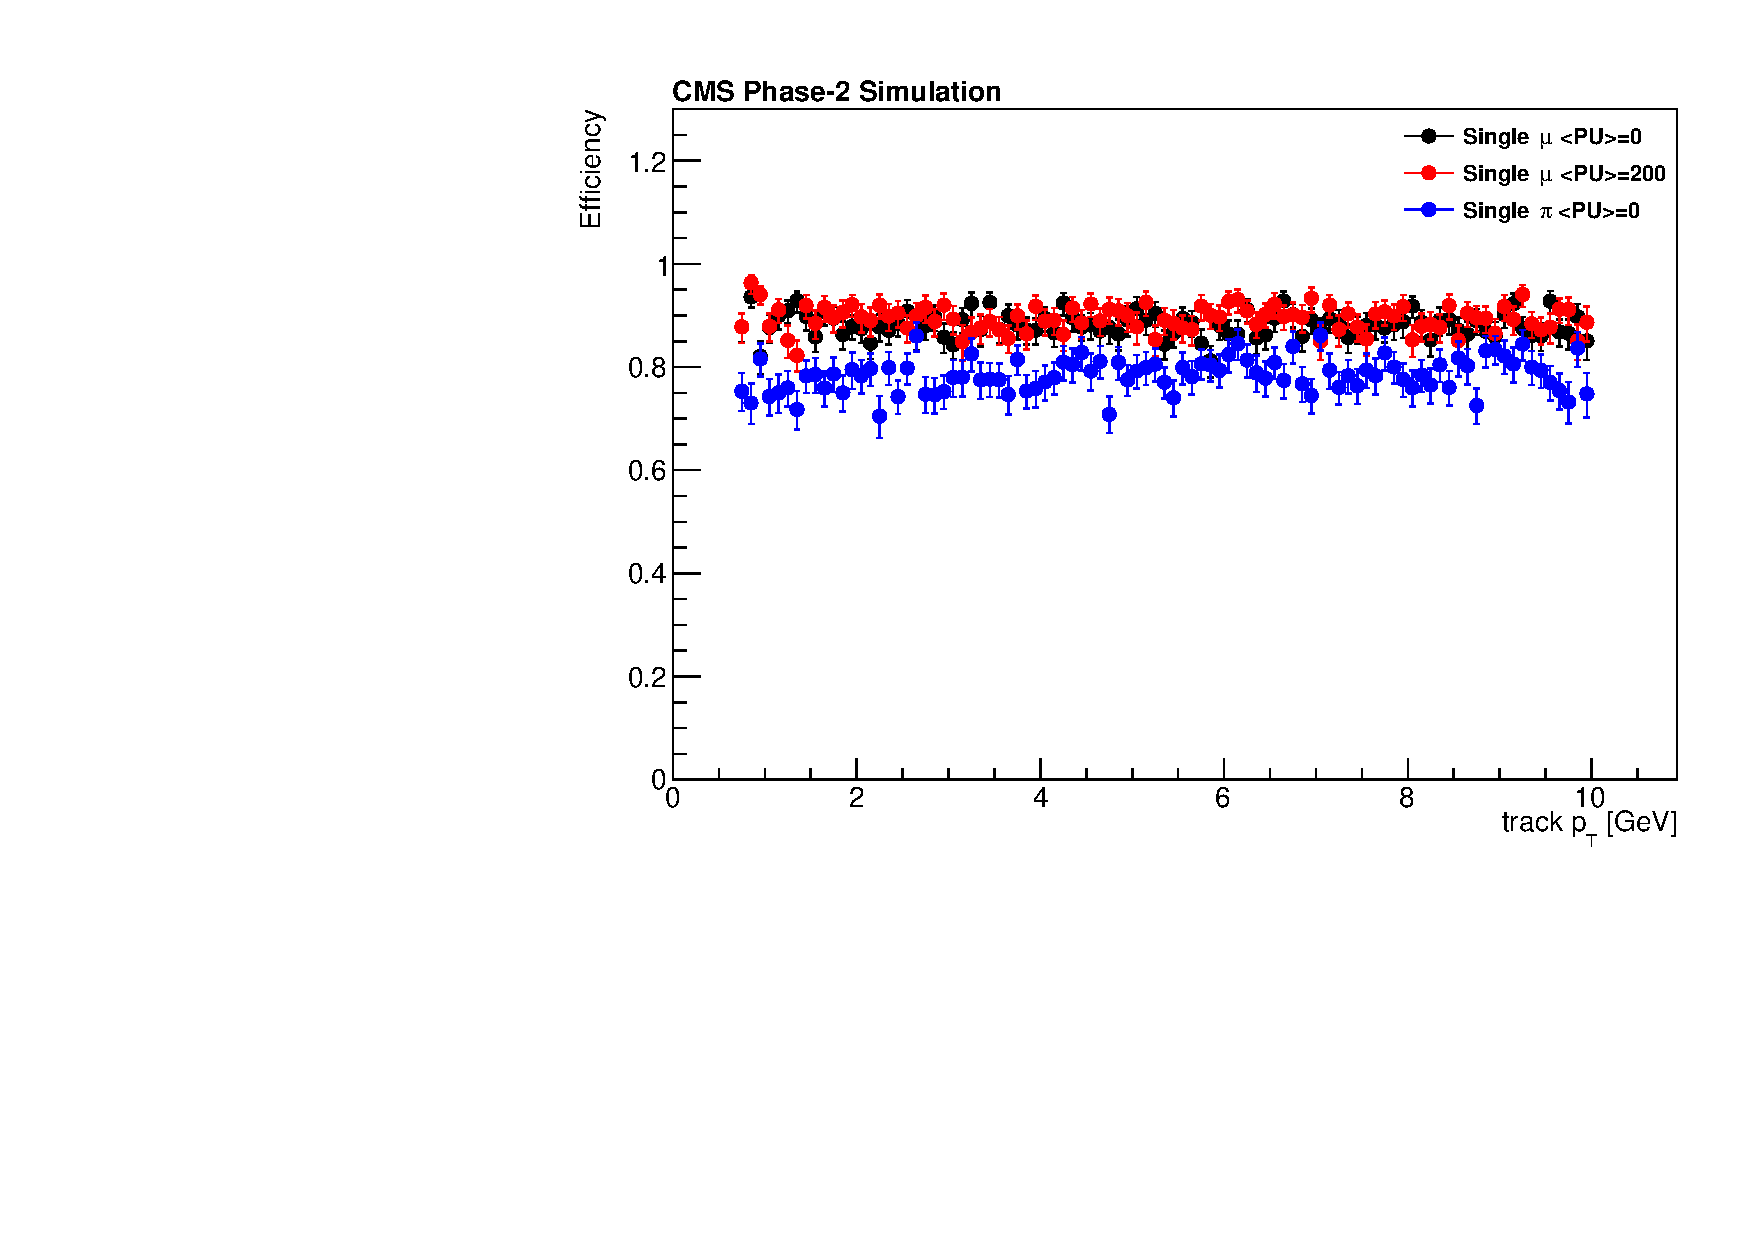
\includegraphics[width=0.48\textwidth]{fig/performance/ClusterAndTracks/divide_mtdTrack_pt_by_track_pt_mupiPUcomp.pdf}
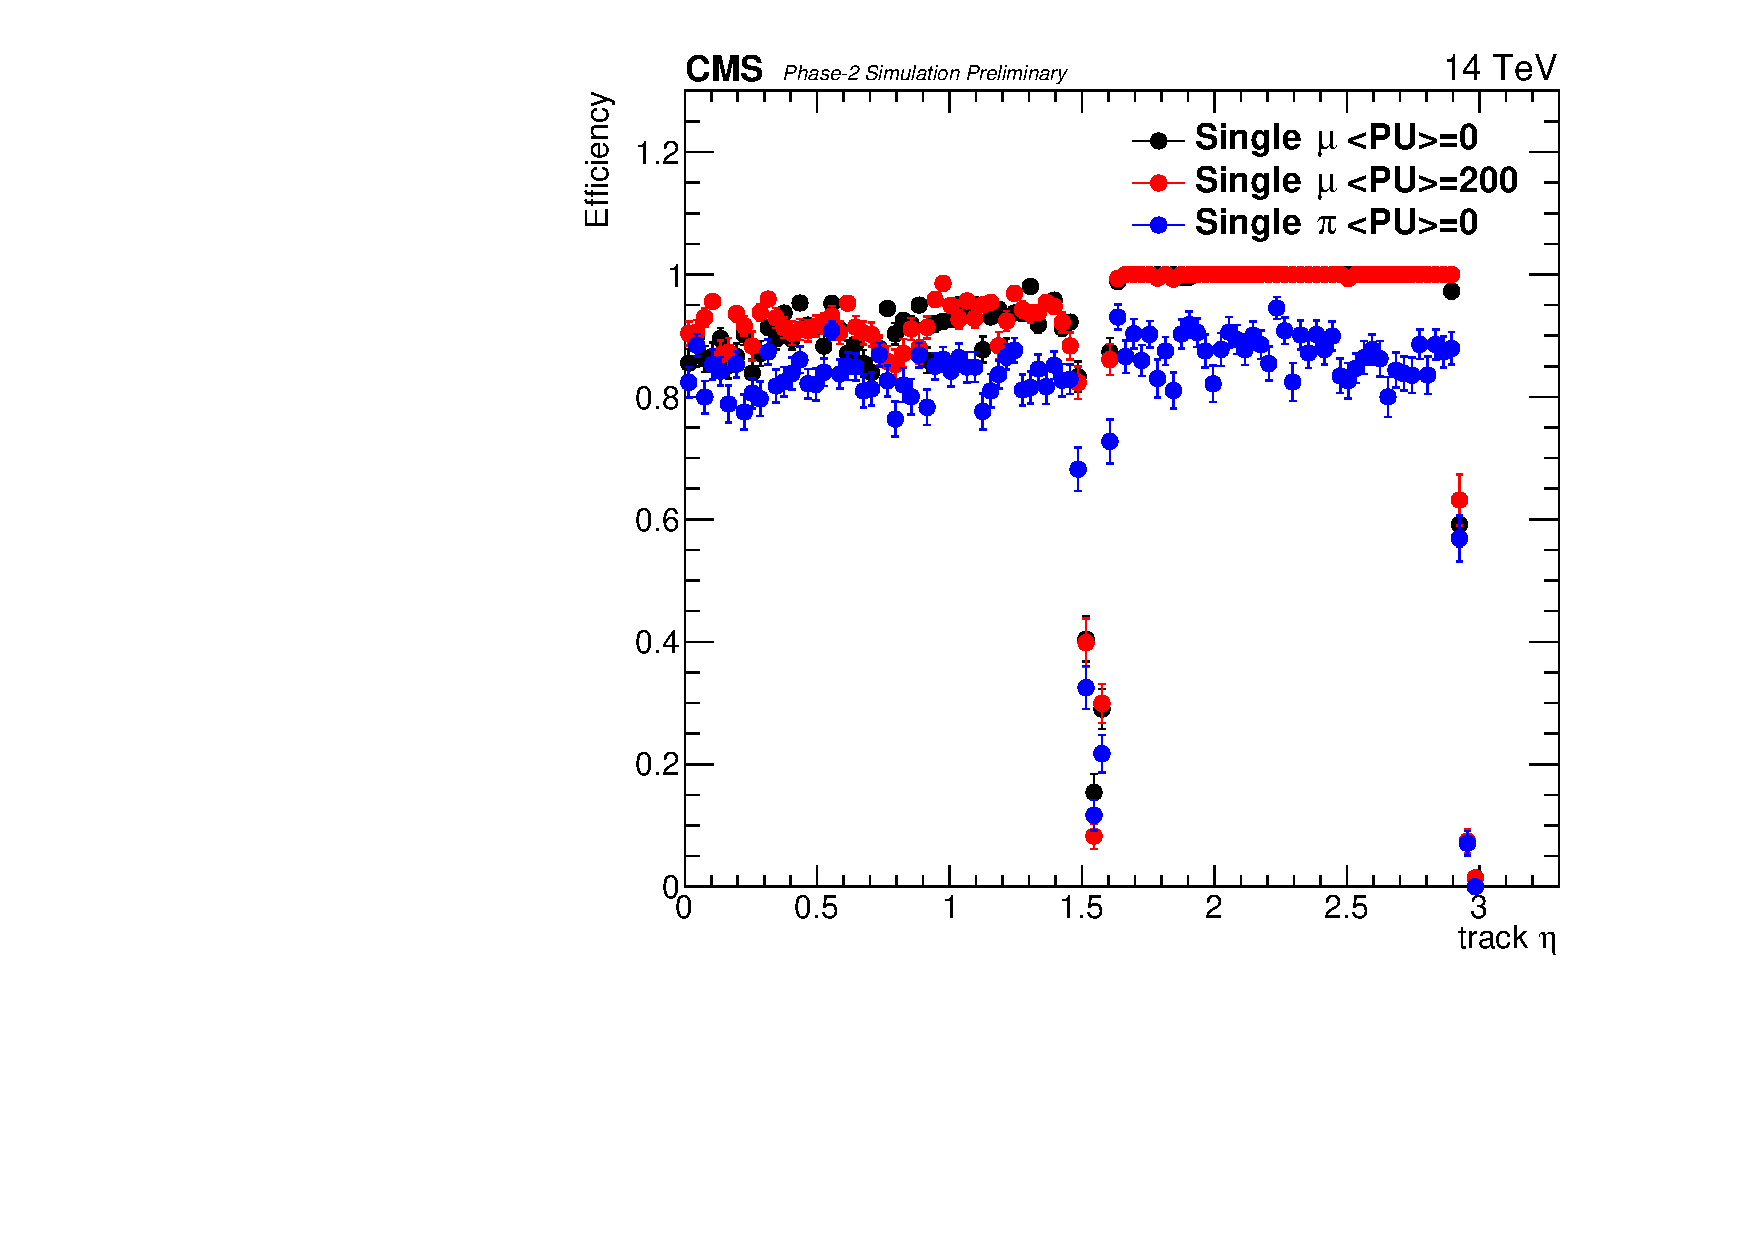
\includegraphics[width=0.48\textwidth]{fig/performance/ClusterAndTracks/divide_mtdTrack_eta_by_track_eta_mupiPUcomp.pdf}
\caption{Per-track efficiency to find an associated MTD cluster to a reconstructed track as a function of transverse momentum (left) and pseudo-rapidity (right). Tracks are matched to a generated particle in the event. Simulated particle gun events with a flat $p_T$ spectrum in the 0.7-10\mathrm{GeV} range are used. Muons (black and red dots are for events without pile-up and with average 200 pile-up events respectively) and pions (blue dots) are compared.}
\label{fig:trackclusterefficiency}
\end{figure}

The resulting time associated to the track and back-propagated to the beamline is compared to the simulation truth in Fig.~\ref{fig:trackt0vsgen}, using pions generated in simulated $t\bar{t}$ events at 14~\mathrm{TeV}. Tracks covering the BTL ($|\eta|<1.5$) and ETL ($1.5<|\eta|<3$) acceptance region are shown separately. From a fit to the distributions, the inferred time resolutions are 33~\mathrm{ps} and 35~\mathrm{ps} respectively for BTL and ETL, matching the expected simulated hit time resolutions. This also shows as expected that the track path-length estimation brings a negligible contribution to the time resolution.

\begin{figure}[!hbtp]
\centering
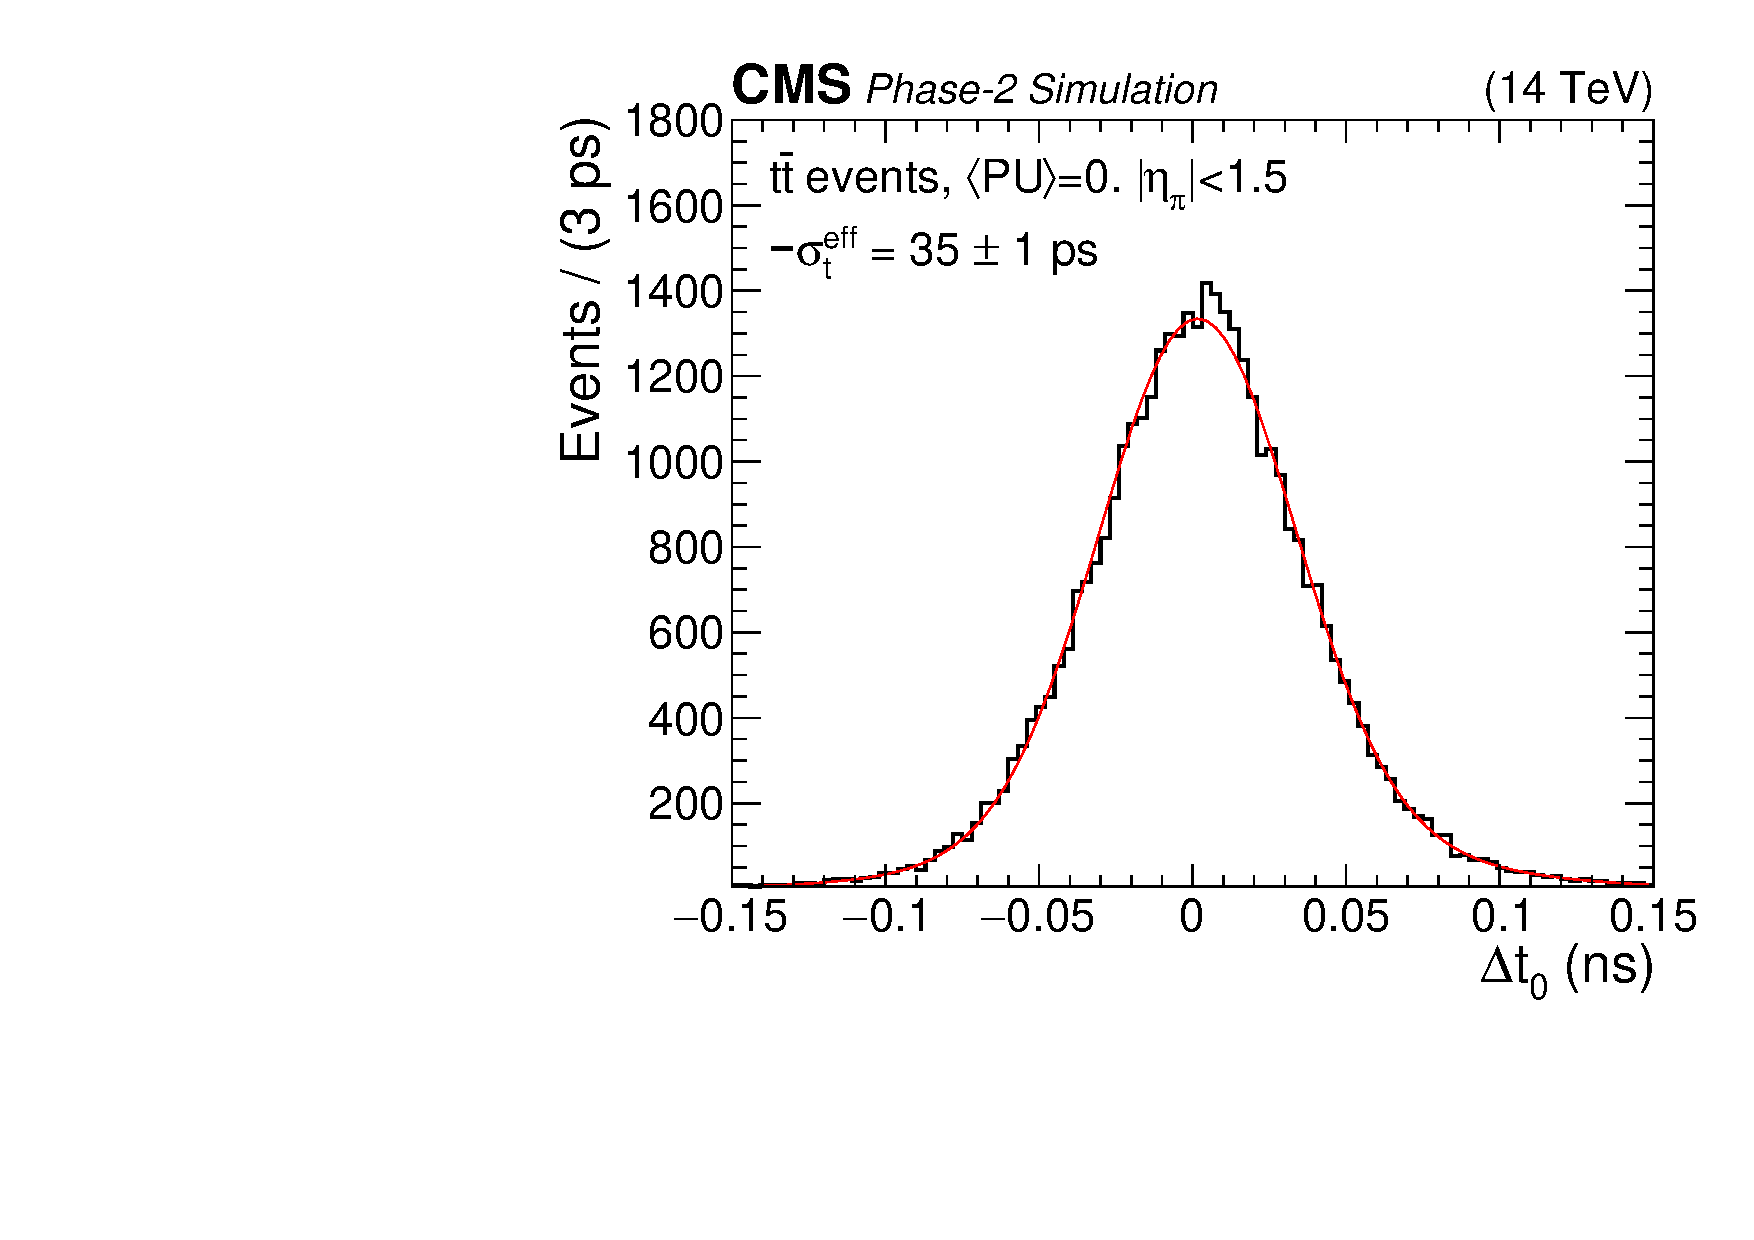
\includegraphics[width=0.48\textwidth]{fig/performance/ClusterAndTracks/res_t_pion_BTL_0PU.pdf}
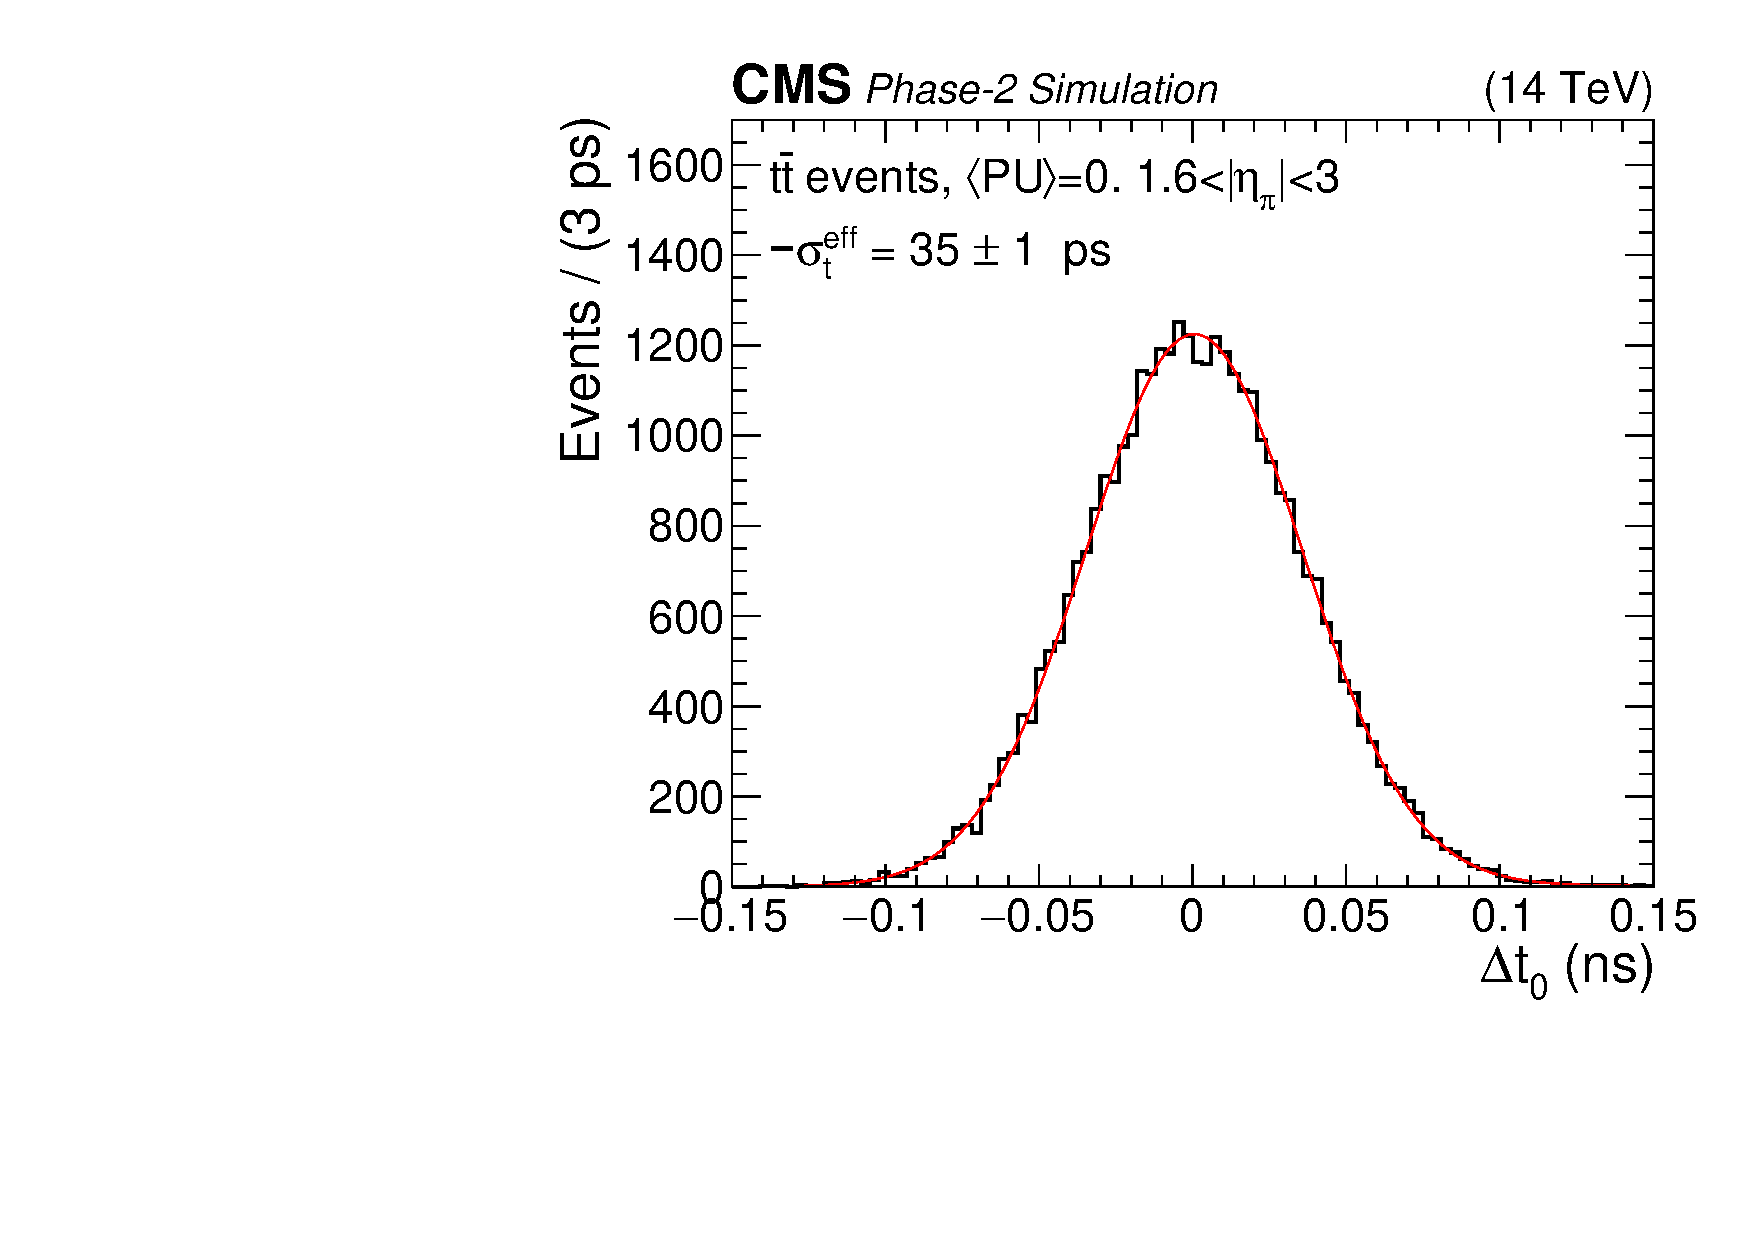
\includegraphics[width=0.48\textwidth]{fig/performance/ClusterAndTracks/res_t_pion_ETL_0PU.pdf}
\caption{Reconstructed track time at vertex respect to the simulation truth. Pions generated in simulated $t\bar{t}$ events at 14~\mathrm{TeV} are used. BTL (left) and ETL (right) acceptance regions are shown separately.}
\label{fig:trackt0vsgen}
\end{figure}

Time resolution for PU200 events in Fig.~\ref{fig:trackt0vsgen_PU200}, shows no degration of the achieved time resolution, with similar performance to the PU0 conditions.

\begin{figure}[!hbtp]
\centering
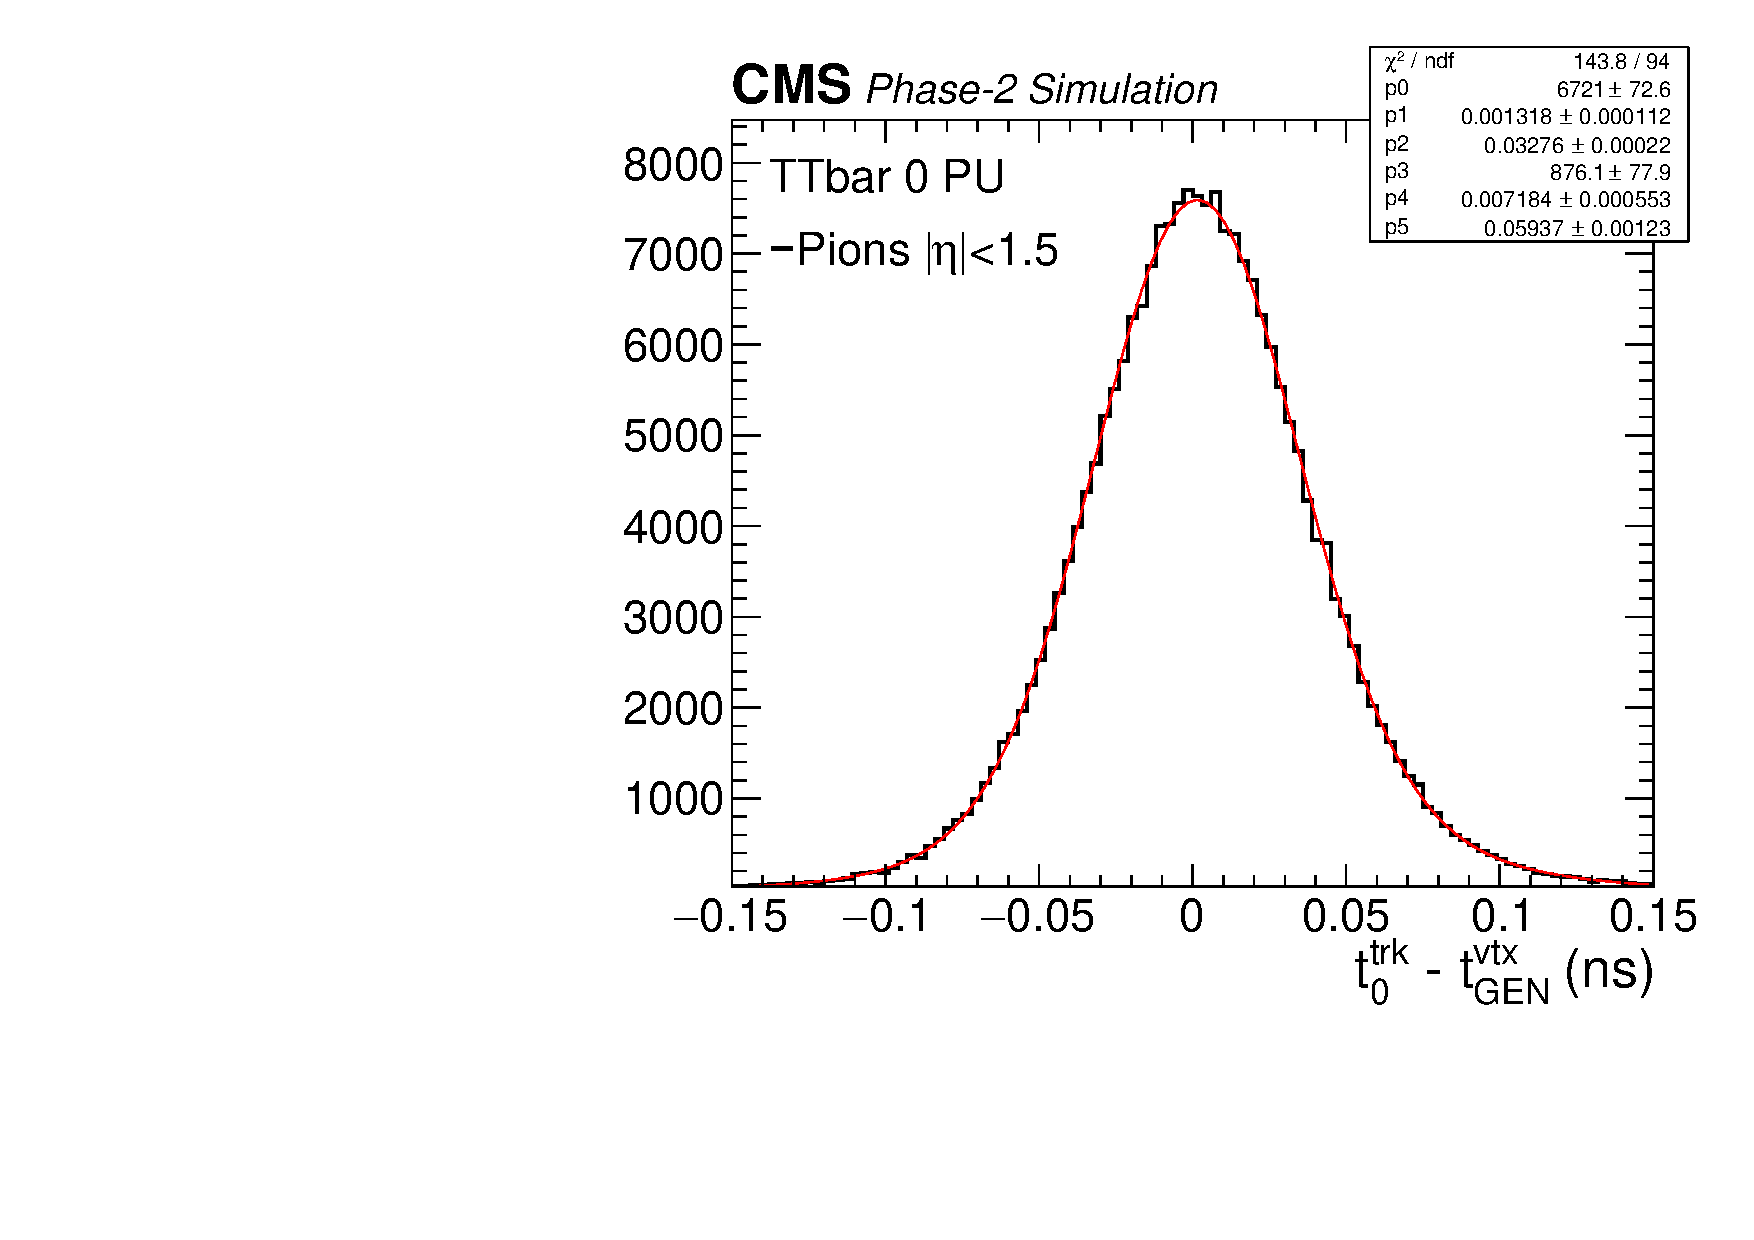
\includegraphics[width=0.48\textwidth]{fig/performance/ClusterAndTracks/res_t_pion_BTL.pdf}
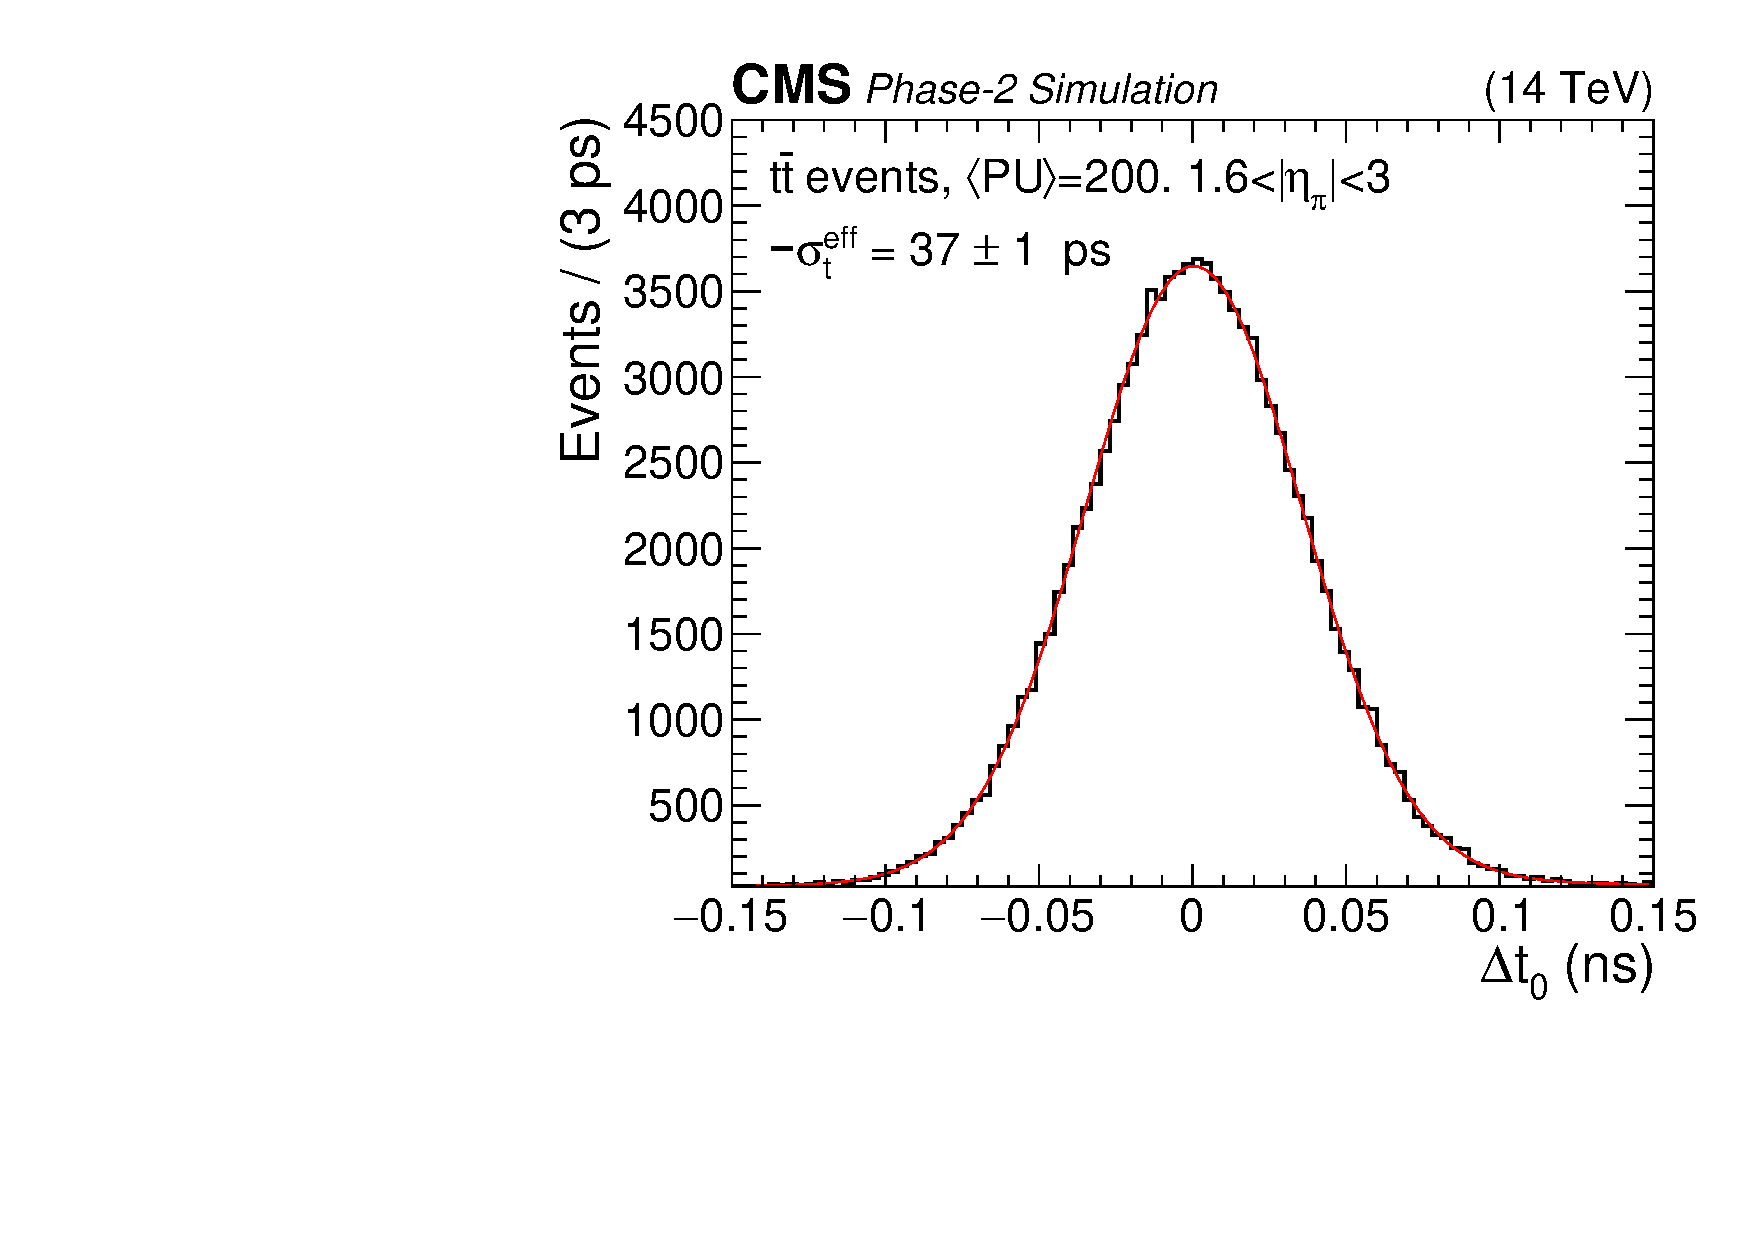
\includegraphics[width=0.48\textwidth]{fig/performance/ClusterAndTracks/res_t_pion_ETL.pdf}
\caption{Reconstructed track time at vertex respect to the simulation truth. Pions generated in simulated $t\bar{t}$ events at 14~\mathrm{TeV} with an average of 200 pile-up events are used. BTL (left) and ETL (right) acceptance regions are shown separately.}
\label{fig:trackt0vsgen_PU200}
\end{figure}

MTD fake hit association has been studied in DYJets events both without pile-up and at PU200. As we have seen fake associations are not an issue for muon tracks which have a precise determination of the extrapolated position at the MTD surface (as signalled by having the same association efficiency for PU0 and PU200 events in Fig.~\ref{fig:trackclusterefficiency}). Fake associations instead have a larger impact for low $p_{T}$ charged hadron tracks, as they typically have shorter tracks, with larger spatial extrapolation uncertainties at the MTD surface.


In order to overcome this issue, different possibility for the hit association has been studied, foreseeing a possible iterative reconstruction for the MTD. Infact, knowing the time of vertex closest to the beam line propagation of the track, it is possible to infer using the track path-length the expected time at BTL. This allows to derive a time compatibility criteria which can be used for the hit association in addition to the space compatibility with the extrapolated track. In absence of the precise time determination for the vertex, the beam spot parameters can also be used as a constraint in the first reconstruction iteration, already with a substantial reduction of the combinatorics for PU200 events. Different mass hypothesis ($\pi,K,p$) can be considered to compute the track velocity when computing the time compatibility; the best mass hypothesis is used to define the matching criteria. 

In order to sort the hits a weighted $\chi^2=\chi^2_{space}+W\times\chi^2_{time}$ with $W=3$ is used. MTD matched tracks are defined to have with $\chi^2_{time}<5$ and  $\chi^2_{space}<50$. The weight $W$ and the matching criteria can be further optimised in the future, making them dependent on the track parameters ($p_{T},\eta,n_{hits},\dots$).  

Figure~\ref{fig:fakes} (left) shows the track-MTD association probability per track to have a good MTD matching (requiring that the back-propagated  time to be within 3$\sigma$ from the vertex time) as a function of $\eta$. Tracks are taken from  from DY events without pile-up and with PU200 and are required to have $p_{T}>0.7$~GeV and to be matched to a generator level particle. No requirement is applied to the track-quality. Different matching criteria are compared, showing that the fraction of tracks for which a good matching MTD hit has only a minor dependence on the matching criteria (somewhat indicating that for good reconstructed tracks the spatial matching is sufficient to identify the MTD hit position). The efficiency to associate the MTD hit remains unchanged going from PU0 to PU200, indicating that the occupancy of the MTD detector allows a good time reconstruction also in the high pile-up environment.   Figure~\ref{fig:fakes} (right) shows the probability per track to have a wrong MTD hit association (back-propagated time above 3$\sigma$ from the vertex time). The different criteria shows a very different performance indicating that the vertex constraint play an important role in the reduction of the fake hits association in high pile-up environment. At the initial reconstruction step a beam spot constraint can be applied (the red-line) already with a large reduction of the fakes. A vertex constraint (blue line) can be applied in a second reconstruction step, perhaps applied only to the tracks sufficiently close to the primary vertex position in high pile-up environment and using the time of the closest reconstructed vertex position (in this study a 3mm cut is applied in the longitudinal direction). With a vertex constraint, both the association efficiency and fake rate can be maintained to levels which are close between PU0 and PU200.

\begin{figure}[!hbtp]
\centering
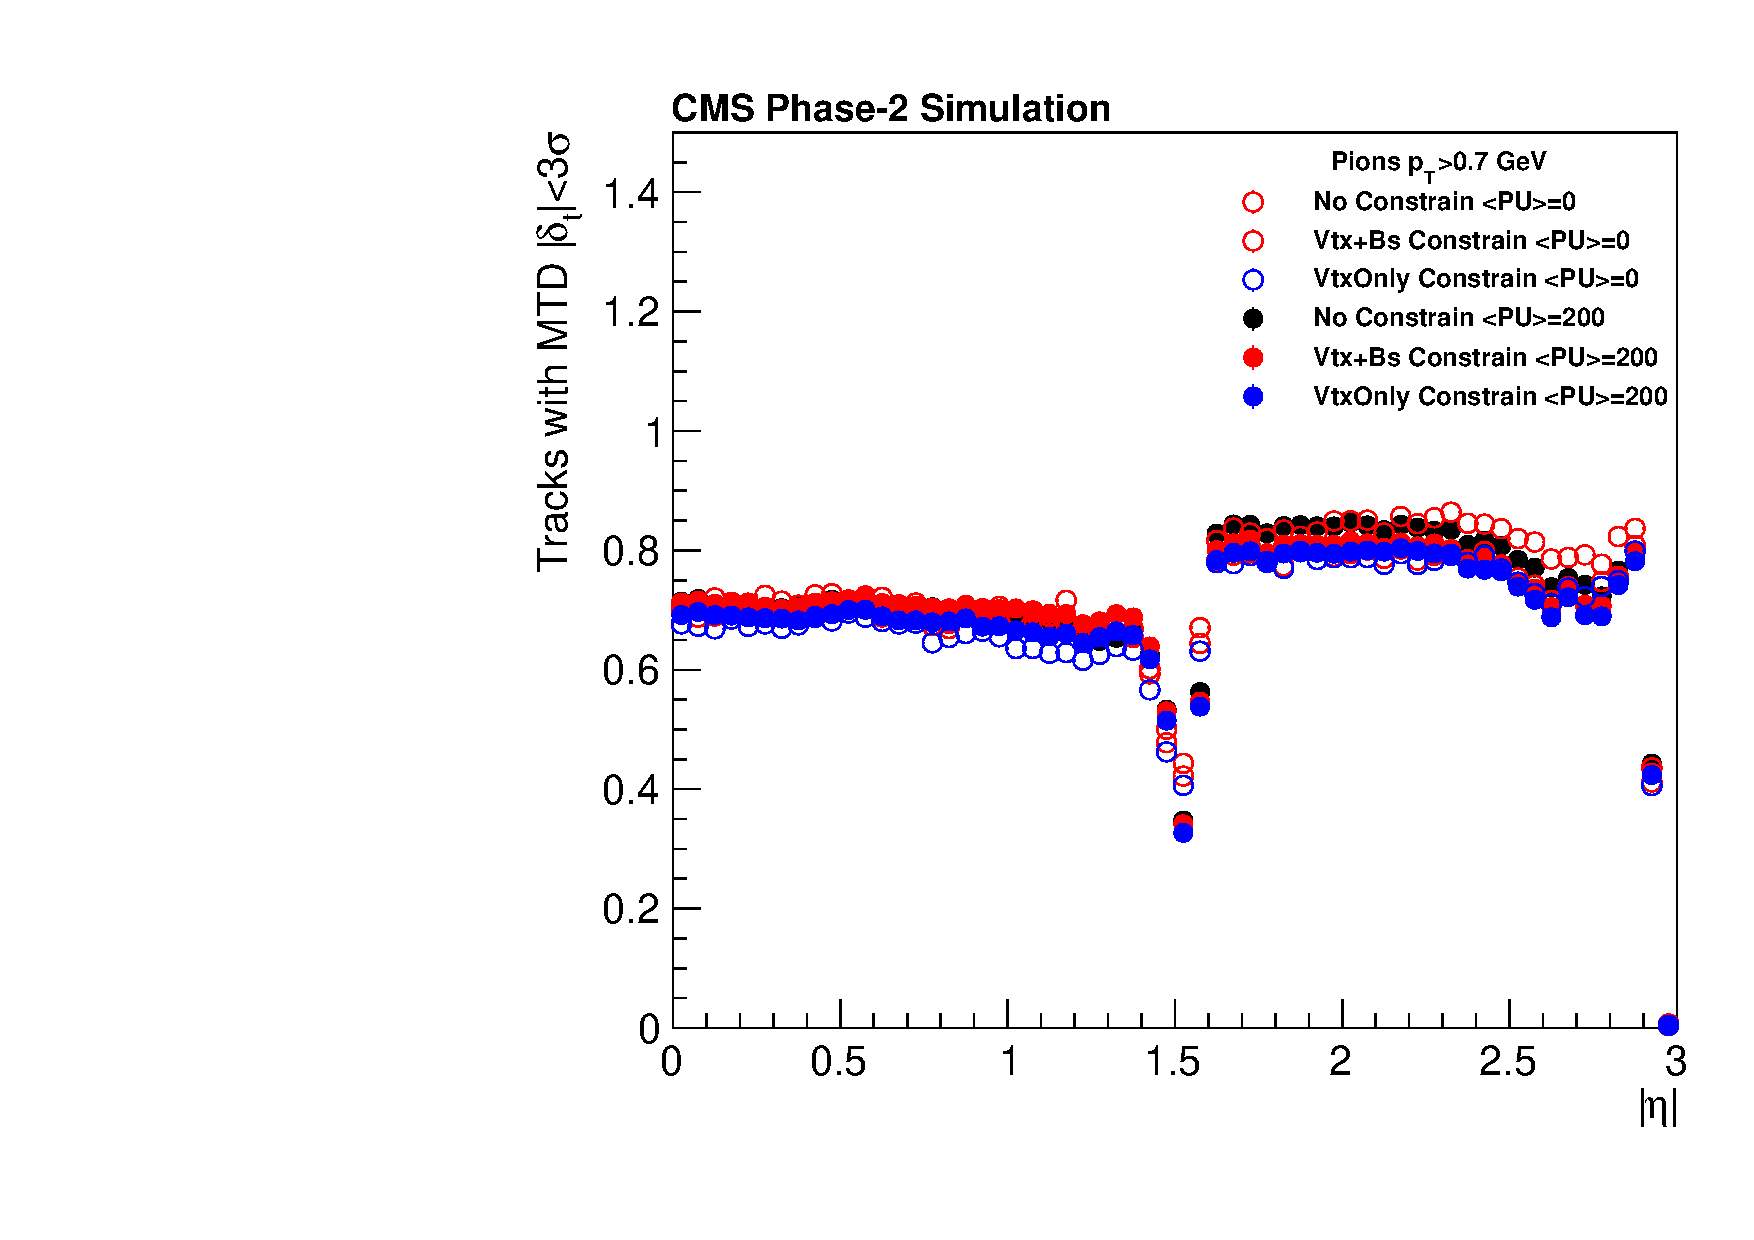
\includegraphics[width=0.48\textwidth]{fig/performance/goodTracks_vs_eta_fullComp.pdf}
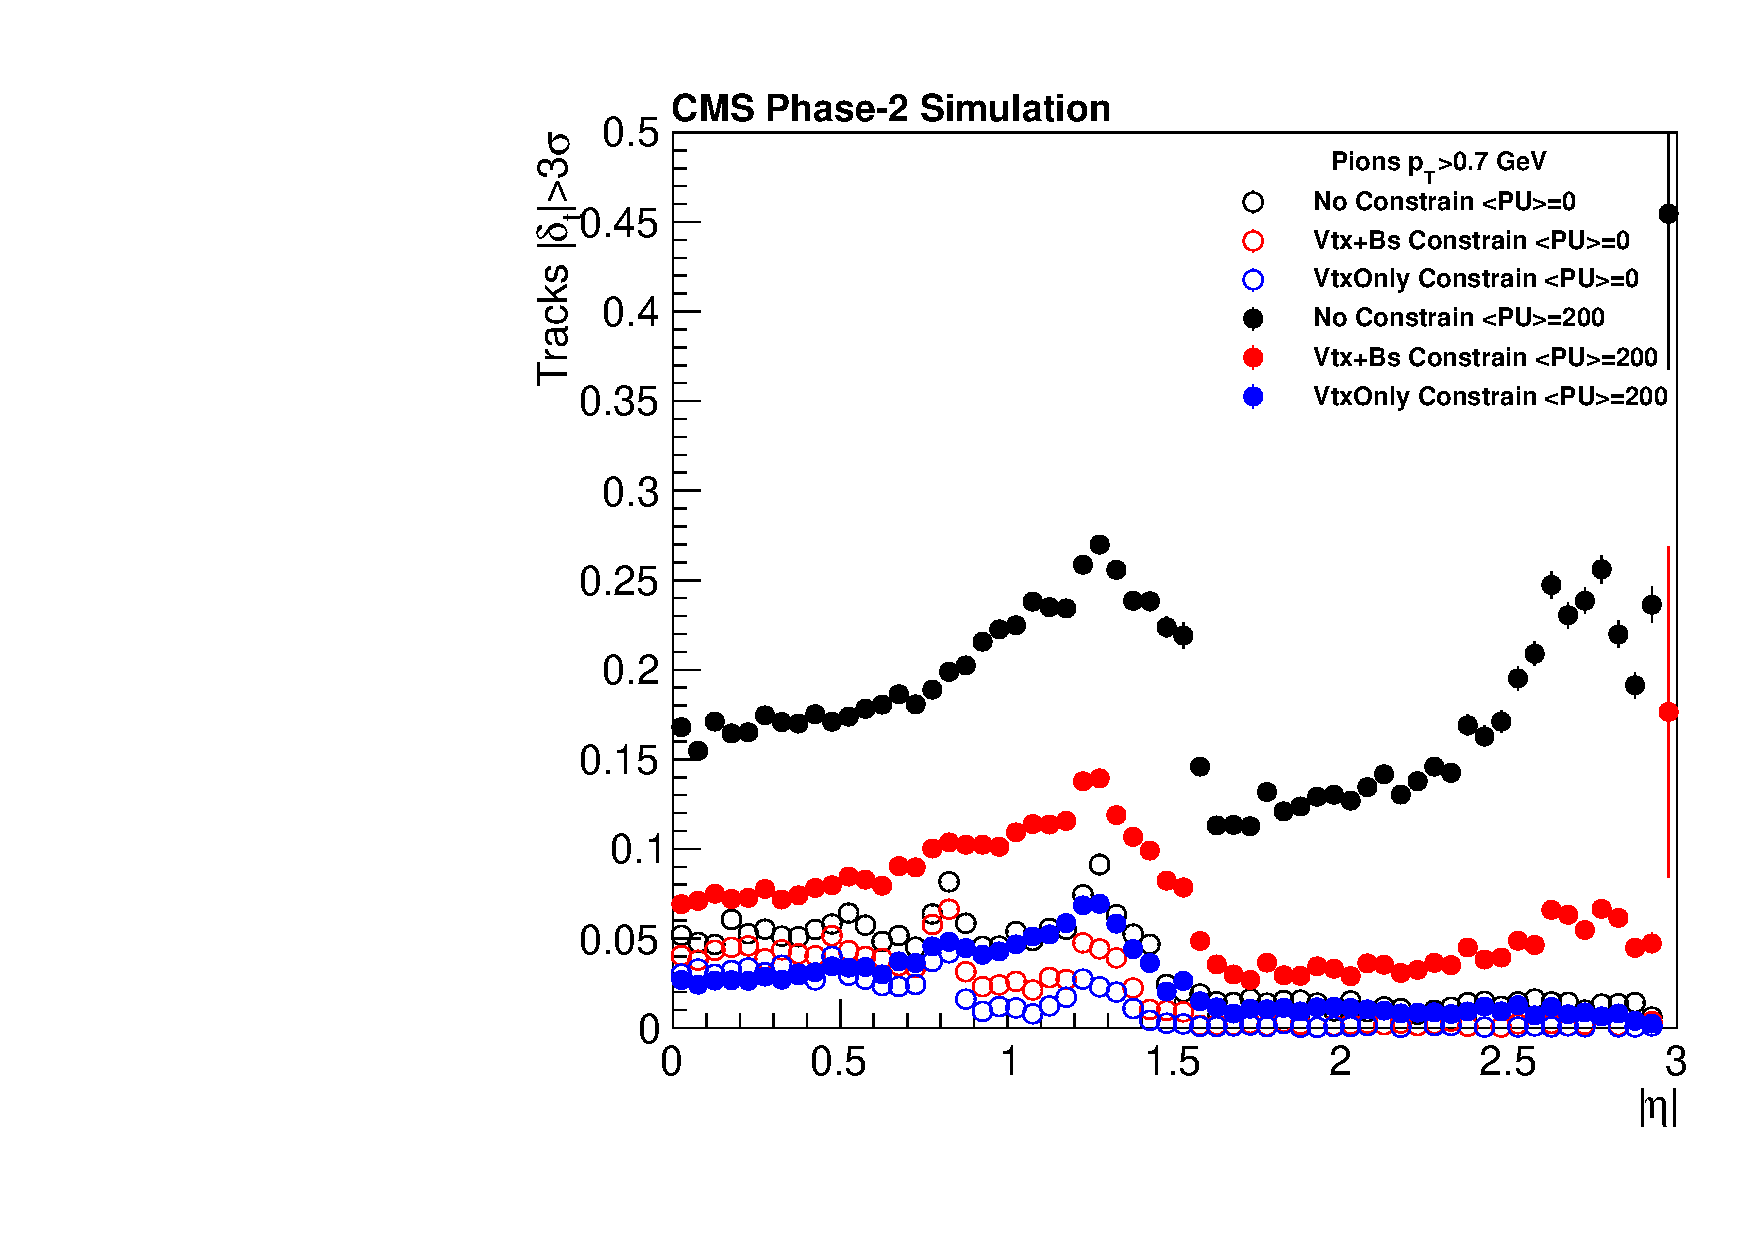
\includegraphics[width=0.48\textwidth]{fig/performance/fakes_vs_eta_fullComp.pdf}
\caption{Probability per track as a function of the pseudo-rapidity to find a good hit association with MTD ($\delta_{t}^{vtx}<3\sigma$, left) and a wrong hit association ($\delta_{t}^{vtx}>3\sigma$, right). Tracks are taken from  from DY events without pile-up and with PU200 and are required to have $p_{T}>0.7$~GeV and to be matched to a generator level particle. No requirement is applied to the track-quality. Different matching criteria are used: black only spatial matching, red time and space matching with a beam spot constrain, blue time and space matching with vertex constrain. See text for more details}
\label{fig:fakes}
\end{figure}

Fake rates are also shown as a function of track $p_{T}$ (left) and track number of hits (right) in Fig.\ref{fig:fakes_pt_nhits}. This shows that the fake rate is not an issue when track extrapolation has a good precision, indicating that the fakes can be further reduced from an optimisation of the track reconstruction at PU200 focussed on low $p_{T}$ hadrons. 

\begin{figure}[!hbtp]
\centering
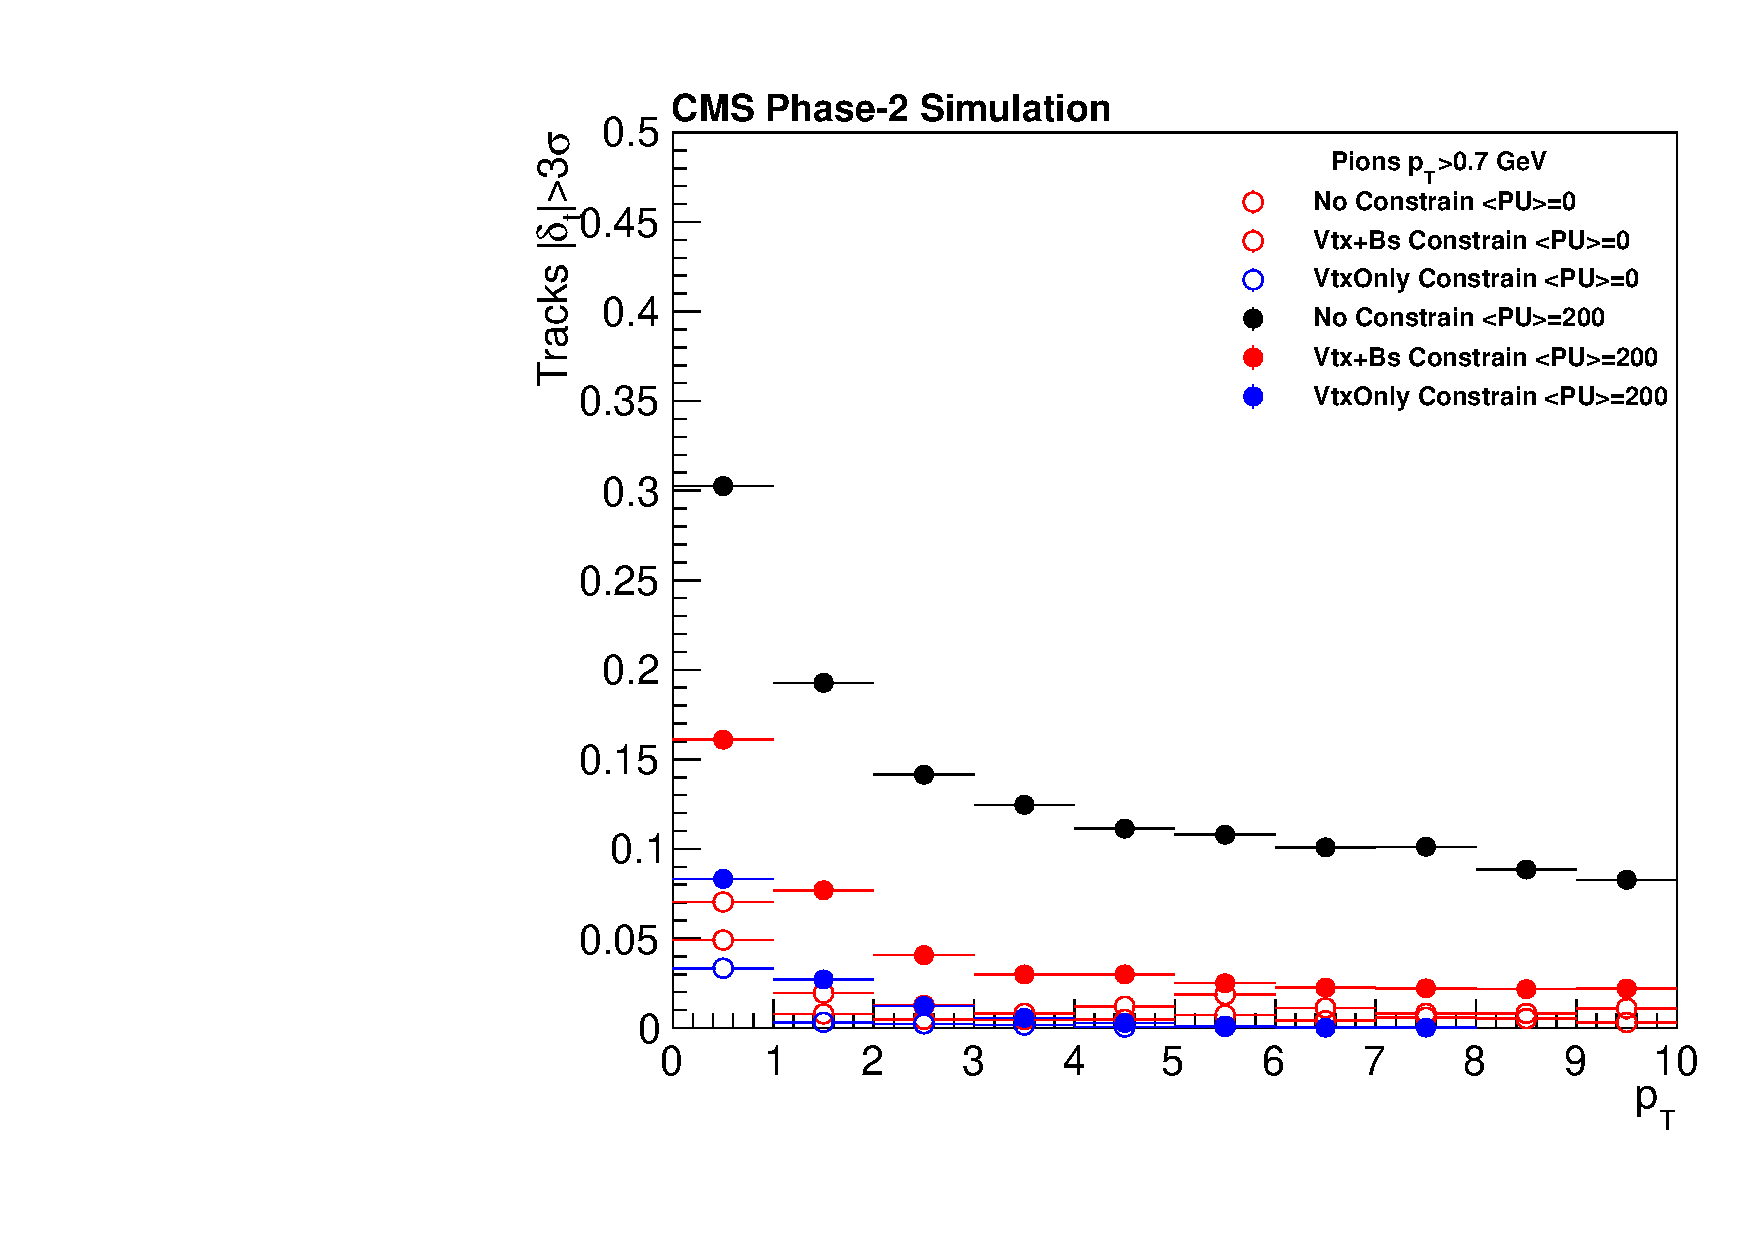
\includegraphics[width=0.48\textwidth]{fig/performance/fakes_vs_pt_fullComp.pdf}
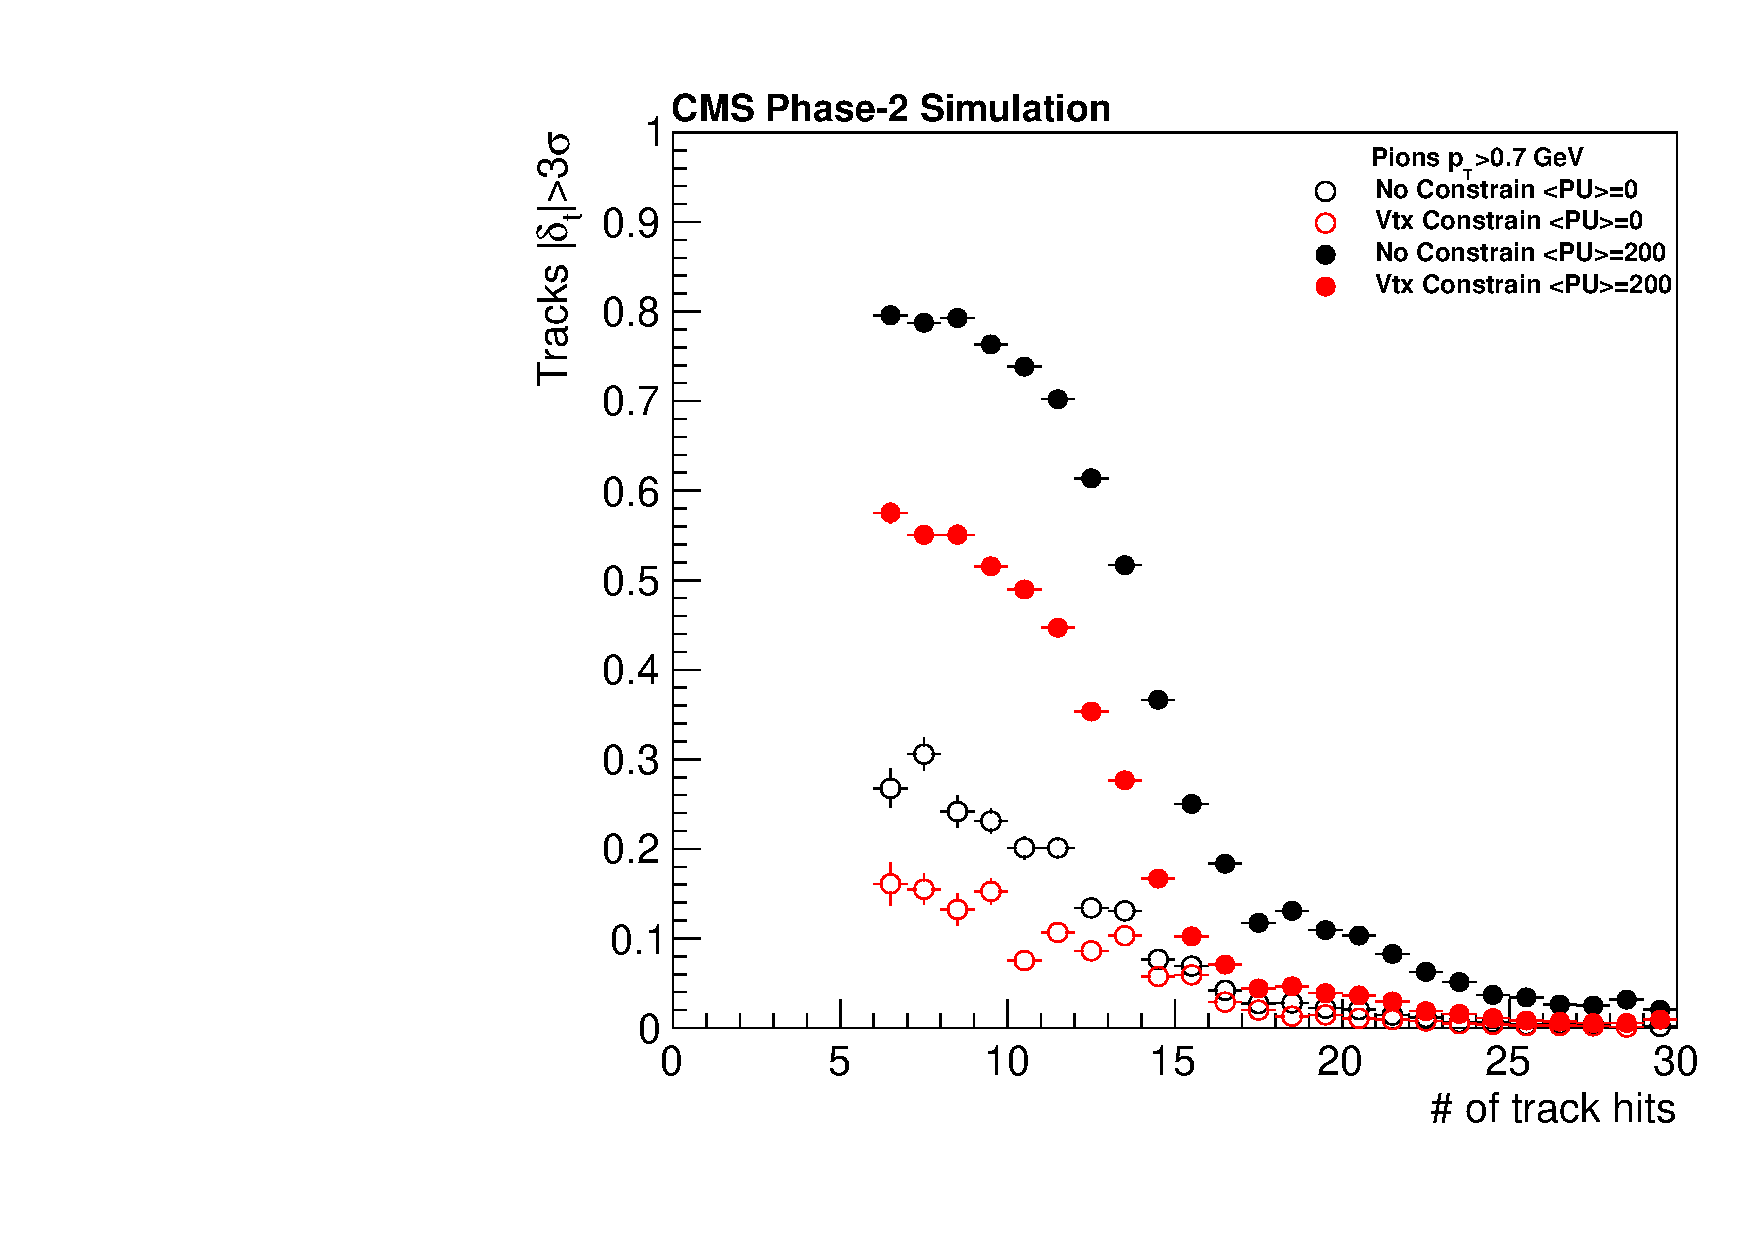
\includegraphics[width=0.48\textwidth]{fig/performance/fakes_vs_nHits.pdf}
\caption{Probability per track as a function of the $p_{T}$ (left) and number of track hits (right) to have a wrong association with MTD ($\delta_{t}^{vtx}>3\sigma$). Tracks are taken from  from DY events without pile-up and with PU200 and are required to have $p_{T}>0.7$~GeV and to be matched to a generator level particle. No requirement is applied to the track-quality. Different matching criteria are used: black only spatial matching, red time and space matching with a beam spot constrain, blue time and space matching with vertex constrain. See text for more details}
\label{fig:fakes_pt_nhits}
\end{figure}

For analysis purposes, tracks can be selected to further reduce the fake contributions (e.g requiring a minimum number of hits). As we will see in the PU rejection studies, these criteria can be further developed implementing a multivariate classifier, feeded with track quality variables and track-MTD matching criteria.

